\section{Reiezione di Banda o Notch}
L'ultimo filtro analizzato, e quello che più ci ha dato filo da torcere nell'analisi, è stato quello a reiezione di banda.

La struttura del filtro notch, riportata in Fig. \ref{fig:circuito}, attenua l'ampiezza di segnale solo per una determinata frequenza, detta anche in questo caso di risonanza ($\nu_0=\frac{1}{2 \pi \sqrt{LC}}$), alla quale la serie di capacità e induttanza avrà impedenza complessiva nulla. Considerando come valori di $R$, $L$ e $C$ le stesse del circuito passa banda, riportiamo le leggi teoriche calcolate:\\

\noindent
\begin{minipage}{.5\linewidth}
\begin{equation}
\frac{|V_{out}|}{|V_{in}|}=
\label{notchGain}
\end{equation}
\end{minipage}%
\begin{minipage}{.5\linewidth}
\begin{equation}
\phi=arctan\left[\frac{R}{\omega L-\frac{1}{\omega C}}\right]
\label{notchPhi}
\end{equation}
\end{minipage}
\break

Come osserviamo dal diagramma di Bode per questo circuito, la legge teorica non è compatibile per alte frequenze in nessuno dei due grafici. I dati sembrano infatti seguire una legge ben diversa da quella stimata. Pertanto inizialmente abbiamo risolto analiticamente il circuito considerando anche la resistenza parassita interna all'induttanza. La legge ricavata ha ridotto la discrepanza tra previsione teorica e dati sperimentali solo per le frequenze vicine a $\nu_0$, ma non ad alte frequenze.

Le formule ricavate sono le seguenti:\\

\noindent
\begin{minipage}{.5\linewidth}
\begin{equation}
\frac{|V_{out}|}{|V_{in}|}=
\label{eq:notchGain_corr}
\end{equation}

\end{minipage}%
\begin{minipage}{.5\linewidth}
\begin{equation}
\phi=arctan\left[
R \frac{\omega L-\frac{1}{\omega C}}{S (R+S)+(\omega L-\frac{1}{\omega C})^2}
\right]\\
\label{eq:notchPhi_corr}
\end{equation}
\end{minipage}
\break

Abbiamo dunque cercato un motivo di tale incompatibilità. Dai dati sembra che per alte frequenze ci sia qualcosa che smorza l'intensità del segnale e ne cambia la fase. Abbiamo dunque avanzato varie ipotesi.

\begin{wrapfigure}[32]{r}[0pt]{115mm}
%	\centering
    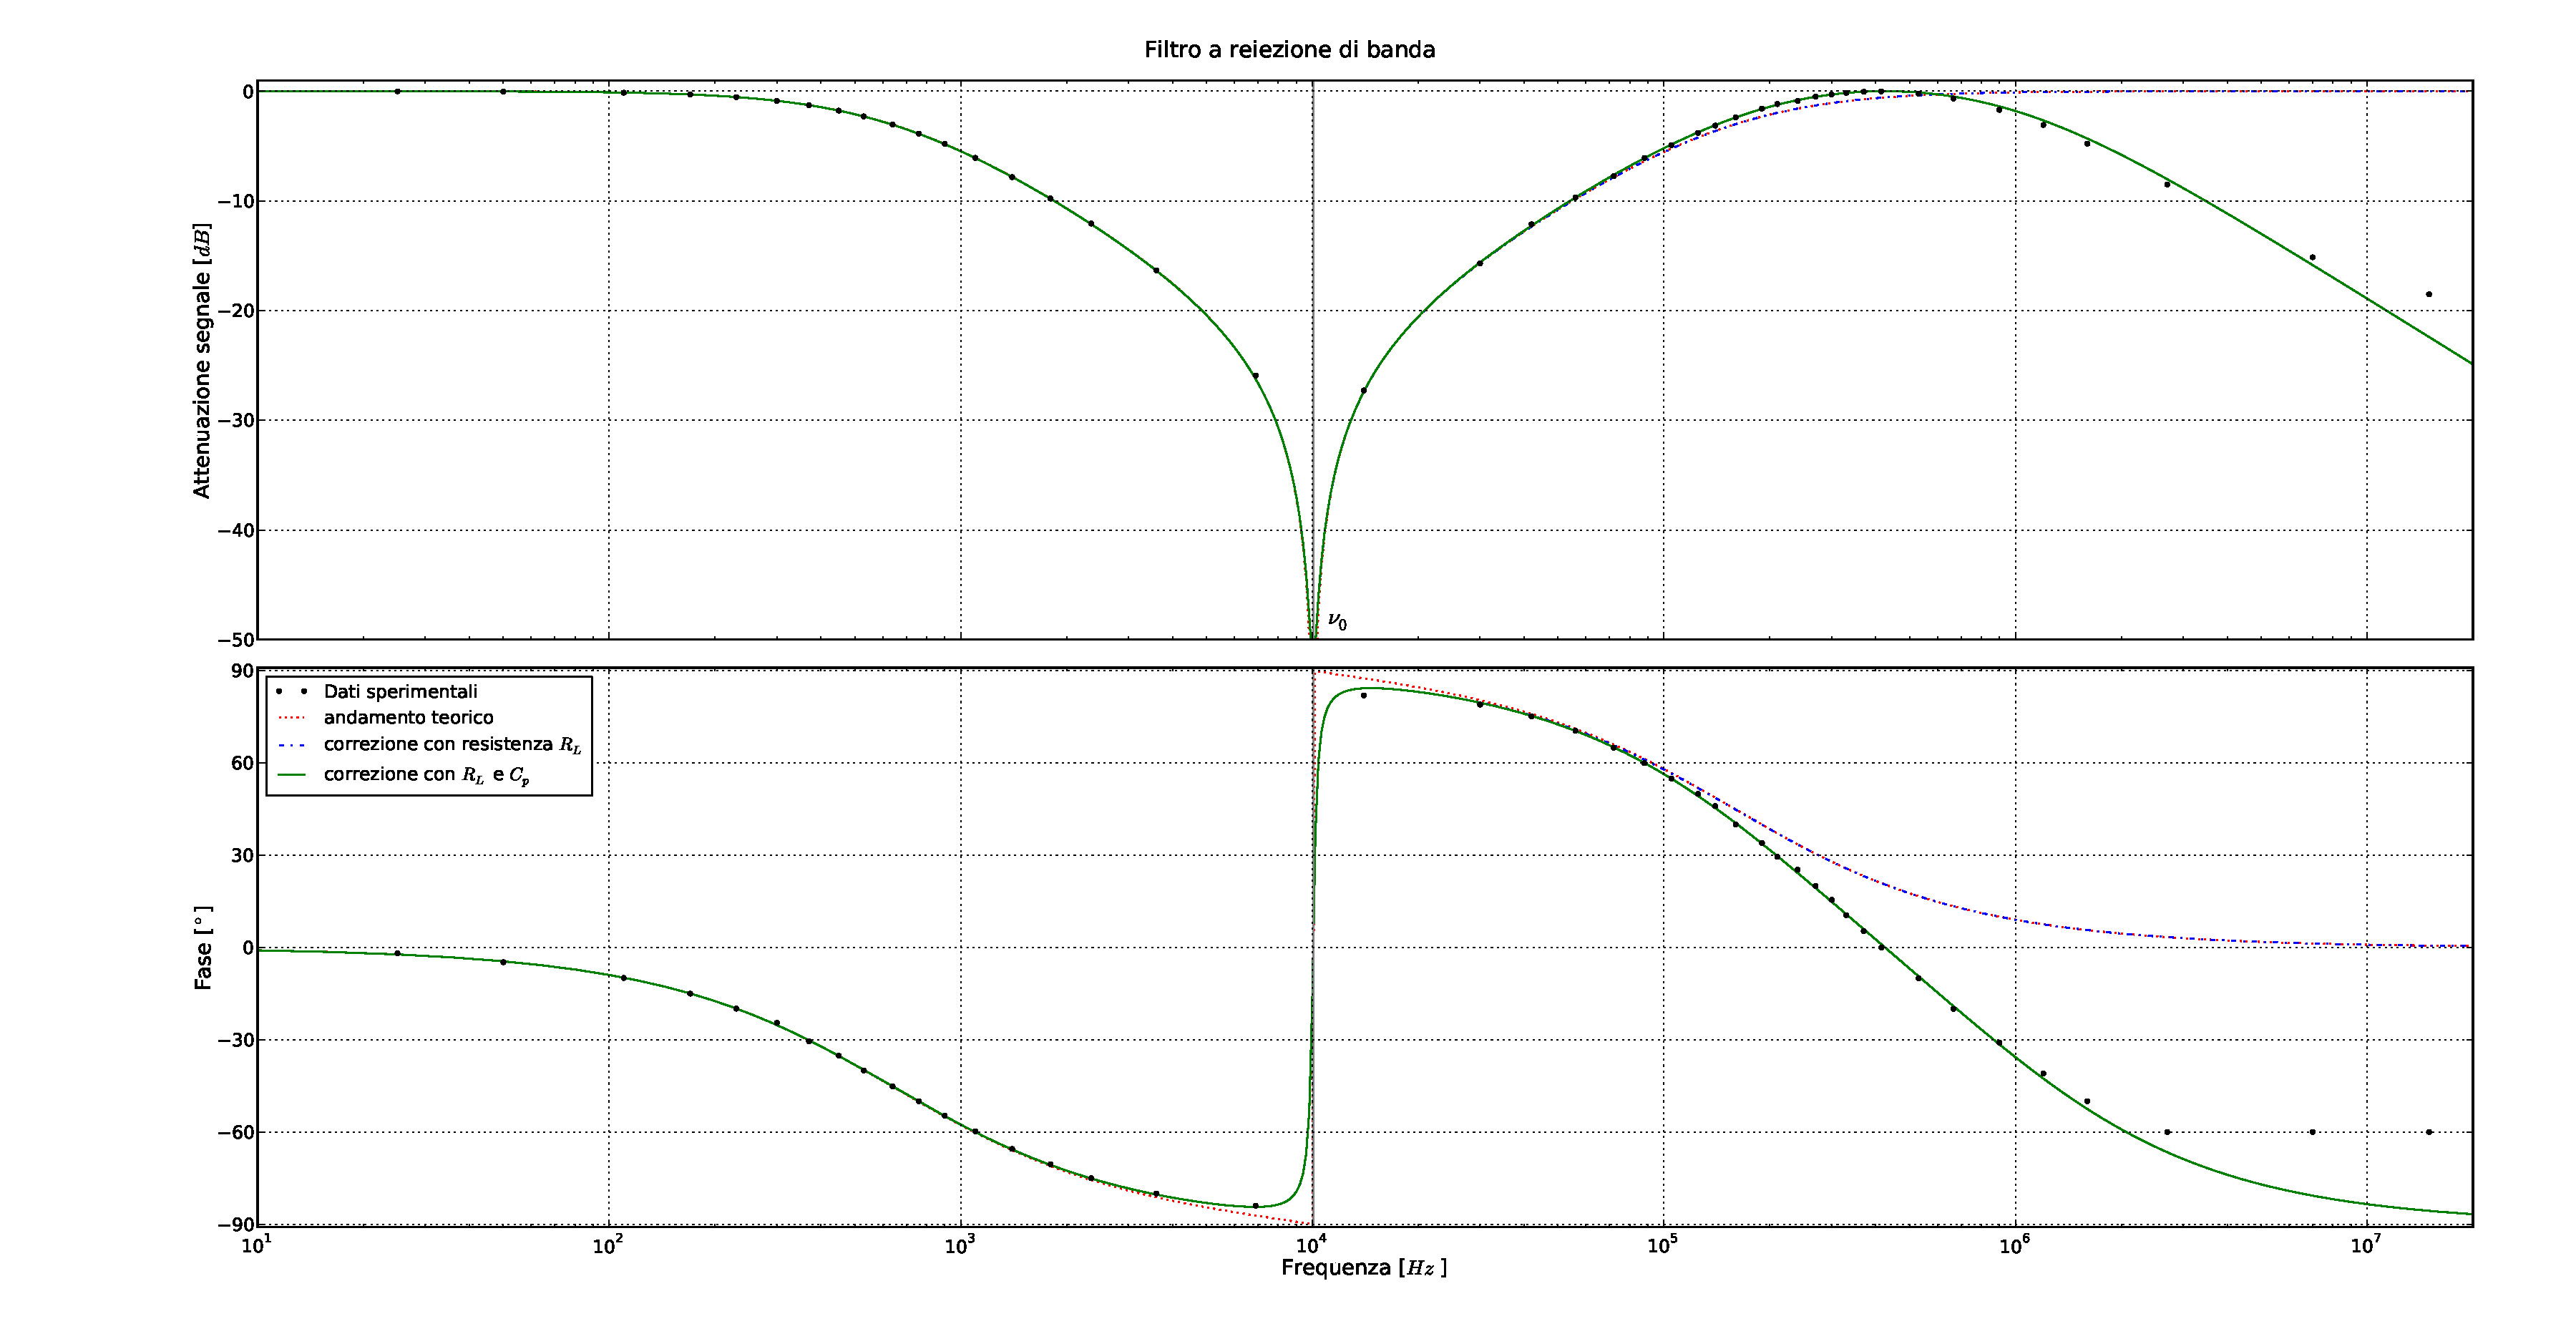
\includegraphics[width=120mm]{notch.pdf}
    \caption{Diagrammi di Bode per il filtro a reiezione di banda.}
    \label{fig:notch}
\end{wrapfigure}

Poiché il comportamento ad alte frequenze è simile a quello del filtro passa basso, la prima ipotesi da noi considerata è stata l'\emph{effetto pelle}. Tale fenomeno si presenta in maniera visibile per lo più ad alte frequenze e consiste nel fatto che la corrente tende a scorrere con più facilità sulla superficie del conduttore (ricordiamo che in regime quasi stazionario la corrente scorre uniformemente all'interno di un conduttore omogeneo e isotropo) che al centro del conduttore. Tale effetto potrebbe causare una capacità parassita. Tuttavia, provando ad aggiungere condensatori in serie al circuito, abbiamo visto subito che essi non causerebbero modifiche nella legge teorica per alte frequenze. Abbiamo dunque escluso l'effetto pelle.

Come seconda ipotesi abbiamo le induttanze parassite dei fili. Infatti, come è noto, ogni filo ho una propria induttanza. Abbiamo dunque risolto nuovamente il circuito mettendo un'induttanza subito prima della resistenza e poi, eseguendo vari plot per diversi valori di induttanza parassita, ne abbiamo analizzato l'andamento. Anche in questo caso l'analisi ha dato esito negativo. Tale correzione infatti non porta un miglioramento di compatibilità con i dati da noi raccolti.

Non sappiamo dunque ancora quale sia la causa di tale discrepanza.